\documentclass[12pt,a4paper]{article}
\usepackage[utf8]{inputenc}
\usepackage[T1]{fontenc}
\usepackage[french]{babel}
\usepackage{graphicx}
\usepackage{amssymb}
\usepackage{geometry}
\usepackage{amsmath}
\usepackage{enumitem}
\usepackage{subcaption}
\usepackage{hyperref}
\usepackage{tikz}
\usetikzlibrary{automata,positioning}

\geometry{hmargin=2.5cm,vmargin=2cm}
\begin{document}
	\begin{flushleft}
	COLLIARD Valentin\\
    \vspace{1\baselineskip}
    TRAORÉ Madina\\
    \end{flushleft}
    \begin{center}
    \vspace{12\baselineskip}
    \begin{huge}
    Rapport\\
    \end{huge}
    \vspace{1\baselineskip}
    \begin{Large}
    Projet :\\
    \textbf{Autour du Google Hash Code 2019\\
    "Photo slideshow"}\\
    \end{Large}
    \vspace{1\baselineskip}
    4I201 - Résolution de problèmes\\
    \vspace{15\baselineskip}
    Master d'Informatique
    \vspace{1\baselineskip}
    \\Ann\'ee universitaire 2018-2019\\
    \vspace{2\baselineskip}
    \includegraphics[scale=0.2]{../../../../logoSorbonne.png}
    \end{center}
    \newpage
    \renewcommand{\contentsname}{\begin{LARGE}
    Sommaire
    \end{LARGE}}
    \vspace*{\stretch{0.5}}
    \noindent\hrulefill
    \vspace{1\baselineskip}
    \begin{large}
    {\setlength{\baselineskip}{1.5\baselineskip}
\tableofcontents\par}
    \end{large}
    \vspace{2\baselineskip}
    \noindent\hrulefill
    \vspace*{\stretch{1}}
    
    \newpage


\noindent L'objectif de ce projet était de résoudre un problème de choix d'ordre de passage
de photos dans une présentation vidéo. Pour cela, nous
avons utilisé diverses techniques
( heuristiques et exactes ) de résolution.

\vspace{1\baselineskip}

\section{Complexité du problème}

\vspace{1\baselineskip}

\noindent \textbf{Montrons que nous pouvons réduire le problème "Photo Slideshow"  au problème de la chaîne hamiltonienne en nous plaçant dans le cas ( plus simple ) où chaque instance ne contiendrait que des photos horizontales}
\vspace{.5\baselineskip}\\
Soit une instance du problème "Photo Slideshow". On peut représenter celle-ci par un graphe $G = (V,E)$ non orienté dont les sommets V correspondent aux différentes photos et les arêtes E aux transitions possibles entre les celles-ci (les transitions étant toutes autorisées, le graphe est complet). S'il existe une présentation pour cette instance c'est-à-dire un ensemble ordonné de photos dans lequel chaque photo est présente une et une seule fois alors il existe dans $G$ une chaîne passant une et une seule fois par chaque sommet du graphe : $G$ contient donc une chaîne hamiltonienne.
\vspace{.5\baselineskip}\\
Soit une instance du problème de la chaîne hamiltonienne représentée par un graphe $G = (V,E)$ non orienté. S'il existe une chaîne hamiltonienne dans $G$ alors cette chaîne est une solution ( présentation ) au problème "Photo Slideshow" si l'on considère que les sommets de $G$ sont des photos.
\vspace{1\baselineskip}\\
Étant donné que le problème de la chaîne hamiltonienne est NP-complet, \textbf{le problème "Photo Slideshow" est bien NP-difficile}.

\vspace{.5\baselineskip}

\section{Techniques de résolution}

\vspace{1\baselineskip}

\subsection{Méthodes gloutonnes}

\vspace{1\baselineskip}

\subsubsection{Méthode proposée}

\vspace{1\baselineskip}

\noindent On remarque rapidement que la méthode gloutonne proposée n'est effectivement pas applicable sur de très grandes instances.\\
Supposons que nous disposons d'une instance contenant $n$ photos. La première photo est choisie de manière aléatoire : il y a donc $n$ possibilités pour celle-ci. Si nous nous plaçons, comme précédemment, dans le cas où l'instance contient uniquement des photos horizontales, l'algorithme glouton proposé va, pour chaque photo, chercher la photo maximisant le score de la transition parmi celles n'ayant pas encore été choisies. Lorsqu'une seule photo a été choisie, il y a donc $n-1$ comparaisons à faire, à la seconde itération il y en a $n-2$ et ainsi de suite. Dans le cas où chaque instance ne contient que des photos horizontales, le complexité de l'algorithme est alors la suivante :
\[\sum_{i=1}^{n-1} i = \frac{n(n-1)}{2}\]\\
Résultats obtenus avec la méthode gloutonne proposée :
\vspace{.5\baselineskip}\\
\verb|b_lovely_landscapes| (1\% de l'instance): 57  \\
\verb|c_memorable_moment| (100\% de l'instance): 1754 \\ 
\verb|d_pet_pictures| (1\% de l'instance): 3714  \\
\verb|e_shiny_selfies| (1\% de l'instance): 3888 
\vspace{1\baselineskip}\\
Il est difficile de juger la qualité de ces résultats - même s'ils semblent prometteurs - puisque nous n'utilisons qu'un faible pourcentage des grosses instances : il est alors possible que nous passions à coté des vignettes et transitions qui donnent de très bons scores. Nous pouvons néanmoins constater que nous obtenons un très bon score sur l'instance \verb|c_memorable_moment| en comparaison au score (152) obtenu lorsque nous avions triés les vignettes horizontales puis verticales.

\begin{figure}[!h]
\centering
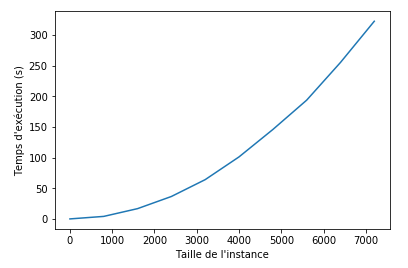
\includegraphics[scale=0.8]{CourbeGlouton1.png}
\caption{Temps d'exécution de la méthode gloutonne proposée en fonction de la taille d'une instance ne contenant que des photos horizontales }
\end{figure}

\subsubsection{Méthode gloutonne plus rapide}

\vspace{1\baselineskip}

\noindent Les résultats obtenus avec la méthode gloutonne proposée paraissant prometteurs nous avons souhaité réutilisé partiellement cet algorithme pour en obtenir un plus rapide. Ce deuxième algorithme glouton fonctionne de la manière suivante : 1 fois sur 2 on choisit la vignette maximisant le score de la transition, le reste du temps la vignette suivante est choisie de manière aléatoire.
\vspace{.5\baselineskip}\\
Résultats obtenus avec cette deuxième méthode gloutonne :
\vspace{0.5\baselineskip}\\
\verb|b_lovely_landscapes| (2\% de l'instance): 114  \\
\verb|c_memorable_moment| (100\% de l'instance): 938 \\ 
\verb|d_pet_pictures| (1\% de l'instance): 2597  \\
\verb|d_pet_pictures| (2\% de l'instance): 5329  \\
\verb|e_shiny_selfies| (1\% de l'instance): 2654\\
\verb|e_shiny_selfies| (2\% de l'instance): 5291 
\vspace{1\baselineskip}\\
Les résultats obtenus sont évidemment moins bons que ceux obtenus précédemment cependant nous sommes maintenant capables d'appliquer l’algorithme sur de plus grosse portion d'instance en un temps raisonnable (deux fois moins de temps qu'avec le premier algorithme).

\begin{figure}[!h]
\centering
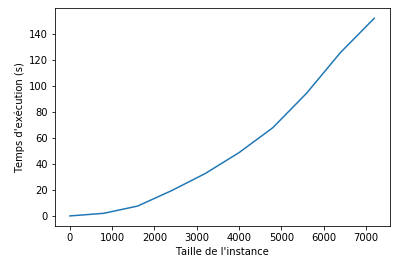
\includegraphics[scale=0.8]{CourbeGlouton2.png}
\caption{Temps d'exécution de la deuxième méthode gloutonne en fonction de la taille d'une instance ne contenant que des photos horizontales }
\end{figure}

\subsubsection{Méthode aléatoire}

\vspace{1\baselineskip}

\noindent Afin de pouvoir juger de la qualité relative de nos solutions et d'avoir une méthode pouvant tourner rapidement sur de très grosses instances nous avons écrit une méthode \textbf{presentationAleatoire} qui construit une solution en rangeant toutes les vignettes de manière aléatoire.
\vspace{.5\baselineskip}\\
Résultats obtenus avec la méthode gloutonne proposée :
\vspace{.5\baselineskip}\\
\verb|b_lovely_landscapes| (100\% de l'instance): 12  \\
\verb|c_memorable_moment| (100\% de l'instance): 141 \\ 
\verb|d_pet_pictures| (100\% de l'instance): 175802  \\
\verb|e_shiny_selfies| (100\% de l'instance): 112459
\vspace{1\baselineskip}\\
On note que ces résultats ont tous été obtenus en moins de 5 minutes et que l'on obtient une solution pour une instance contenant 7000 photos en 0.3 secondes.

\subsection{Méta-heuristiques}

\vspace{1\baselineskip}

\subsubsection{Descente stochastique}

\vspace{1\baselineskip}

\noindent Nous appliquons une descente stochastique après avoir obtenu une solution avec notre deuxième méthode gloutonne. Afin de ne pas avoir un voisinage trop conséquent nous avons choisi de ne permuter que les vignettes consécutives au cours de la descente stochastique. Par ailleurs, on applique une fois sur deux le premier voisinage (permuter deux vignettes consécutives) puis on applique l'autre voisinage (permuter une des deux photos verticales entre deux vignettes) le reste du temps. Le temps d'exécution étant relativement long, on cherche une meilleure solution sur 10 itérations seulement.
\vspace{.5\baselineskip}\\
Résultats obtenus avec notre deuxième méthode gloutonne suivie d'une descente stochastique :
\vspace{.5\baselineskip}\\
\verb|b_lovely_landscapes| (2\% de l'instance): 117  \\
\verb|c_memorable_moment| (100\% de l'instance): 1017 \\ 
\verb|d_pet_pictures| (1\% de l'instance): 2688  \\
\verb|e_shiny_selfies| (1\% de l'instance): 2675
\vspace{1\baselineskip}

\subsubsection{Algorithme génétique}

\vspace{1\baselineskip}

\noindent Ayant auparavant remarqué que l'algorithme génétique fournissait de bonnes solutions pour le problème du voyageur de commerce qui est assez similaire au problème présenté ici, nous avons souhaité tester son efficacité sur l'instance \verb|b_lovely_landscapes| (plus simple à manipuler).\\
En lançant l'algorithme sur 2\% de l'instance avec une population de 20 individus obtenus avec notre deuxième algorithme glouton, sur 100 générations et avec une probabilité de mutation de 0.4, nous obtenons en 1 minute une solution ayant un score de 168 donc meilleur que toutes les autres solutions trouvées jusqu'ici pour cette instance.
 
\subsection{Programmes Linéaire en Nombres Entiers}

\vspace{1\baselineskip}

\noindent Nous avons réadapté le PLNE donné en annexe permettant de résoudre un TSP afin qu'il puisse résoudre notre problème (chaîne hamiltonienne de poids maximum). Pour éviter les sous-boucles dans nos solutions nous avons utilisé les contraintes MTZ qui permettent d'avoir une formulation compacte. On note ici V la liste des vignettes de l'instance, $x_{ij}$ les variables binaires indiquant si la transition (i,j) existe ou non dans la présentation et $u_{ij}$ les variables réelles permettant de gérer les contraintes MTZ.

\vspace{1\baselineskip}

\begin{equation}
\begin{array}{rrclcl}
\displaystyle \max_{} & \displaystyle \sum_{i,j}^{} s_{ij}x_{ij} \\
\textrm{s.c.} &  \displaystyle \sum_{j \in V}^{} x_{ij} & \leq & 1 &  \forall i \in V\\
&  \displaystyle \sum_{j \in V}^{} x_{ji} & \leq & 1 & \forall i \in V\\
&  \displaystyle \sum_{i,j}^{} x_{ij} & = & n-1 \\
& x_{ij}  +  x_{ji} & \leq & 1\\
& & u_{i} = 1 &\\
& 2 & \leq & u_{i} & \forall i \in V\\
& u_i & \leq & n & \forall i \in V\\
& u_i - u_j + 1 & \leq & n(1-x_{ij}) & \forall i,j \in V
\end{array}
\end{equation}
\newpage

\noindent En lançant notre PLNE sur 1\% de l'instance \verb|b_lovely_landscapes| (800 premières images), nous obtenons un score de 57. Le programme tourne pendant environ 5 minutes, mais Gurobi précise que 83 secondes suffisent à trouver une solution.\\
Nous remarquons également que la matrice de scores est creuse. On peut alors supposer que l'instance a été faite de manière à ce qu'il y ait peu de bonnes solutions, ce qui expliquerait les mauvais résultats obtenus avec les algorithmes précédents.

\subsection{Heuristiques d'arrondi}

\vspace{1\baselineskip}

\noindent En appliquant l'heuristique d'arrondi proposée sur 1\% de l'instance \verb|b_lovely_landscapes| nous obtenons le même score qu'avec le PLNE. Cependant le temps d'exécution reste très long. Nous allons donc essayer d'appliquer un algorithme semblable à celui de Kruskal pour avoir une meilleure complexité.

\section{Analyse expérimentale}

\vspace{1\baselineskip}

\noindent Nous avons implémenté deux types de méthodes différentes : d'une part les méthodes très rapides pouvant être executées sur de très grosses instances (algorithme glouton semi-aléatoire et méthode aléatoire). Le problème de ce genre de méthodes est que nous obtenons des scores assez mauvais pour l'instance \verb|b_lovely_landscapes|. La meilleure solution trouvée sur la totalité de l'instance est moins bonne que celles trouvées sur 1\% seulement de l'instance avec les autres algorithmes.
\vspace{1\baselineskip}\\\
D'autre part, nous avons des algorithmes en $O(n^2)$ minimum, qui ne peuvent pas être exécutes sur la totalité des instances fournies. Dans cette catégorie nous retrouvons l'algorithme glouton proposé, le PLNE, l'heuristique d'arrondi et l'algorithme de tri des transitions par scores. En contre partie d'une complexité plus grande, nous obtenons des scores bien plus prometteurs.
\vspace{1\baselineskip}\\
Ainsi nous pouvons conclure qu'aucun algorithme très performant ne peut être exécuté sur de grosses instances. De plus, on peut deviner que certaines instances données ont été construites pour pouvoir donner un très bon score dans peu de cas seulement (notamment \verb|b_lovely_landscapes|) alors que certaines instances donnent de très bons scores même avec des algorithmes aléatoires.
\vspace{1\baselineskip}\\
Pour finir, on remarque que pour de très petites instances, allant jusqu'à quelques milliers de photos, les algorithmes plus précis et demandant plus de ressources sont meilleurs. Cependant, une fois cette limite dépassée, ces mêmes algorithmes ne sont plus utilisables car ils prendront un temps de traitement beaucoup trop long, contrairement à des algorithmes plus randomisés.

\section{Meilleurs résultats obtenus}

\vspace{1\baselineskip}

\noindent Les meilleurs résultats obtenus sont les suivants :
\vspace{1\baselineskip}\\
\verb|b_lovely_landscapes| (2\% de l'instance avec l'algorithme génétique): 168  \\
\verb|c_memorable_moment| (100\% de l'instance avec le premier algorithme glouton): 1754 \\ 
\verb|d_pet_pictures| (100\% de l'instance avec la méthode aléatoire suivie d'une descente stochastique): 216 130 \\
\verb|e_shiny_selfies| (100\% de l'instance avec la méthode aléatoire suivie d'une descente stochastique): 145 605 

\end{document}
